\section{Aufgabe 16}
\subsection{a)}
Entropie berechnen:
\begin{align*}
  S &= - \sum_i p_i\log_2(p_i) \\
    &= - \left[ P(\symup{Fußball=True})\log_2(P(\symup{Fußball=True})) +
        P(\symup{Fußball=False})\log_2(P(\symup{Fußball=False}))\right] \\
    &= 0,9402 \\
\end{align*}

mit
\begin{align*}
  P(\symup{Fußball=True}) &= \frac{9}{14}\\
  P(\symup{Fußball=True}) &= \frac{5}{14}\\
\end{align*}

\subsection{b)}
Informationsgewinn(Wind):
\begin{align*}
  IG(Y|X) &= H(Y)-H(Y|X) \\
  IG(Wind|Fußball) &= S - \frac{|D_{\symup{Wind=True}}|}{|D|} \cdot
                          H(D_{\symup{Wind=True}}) -
                          \frac{|D_{\symup{Wind=False}}|}{|D|} \cdot
                          H(D_{\symup{Wind=False}})\\
                  &= 0,04860\\
\end{align*}
Hierbei ist $S$ die in a) berechnete Entropie, $|D_{\symup{Wind=True}}|$ die
Anzahl der Wind-Einträge mit "True", $|D_{\symup{Wind=False}}|$ die Anzahl der
Wind-Einträge mit "False" und $|D|=14$ die Gesamtanzahl der Einträge,
mit den bedingten Wahrscheinlichkeiten
\begin{align*}
  P(\symup{Fußball=True|Wind=True}) = \frac{1}{2} \\
  P(\symup{Fußball=False|Wind=True}) = \frac{1}{2} \\
  P(\symup{Fußball=True|Wind=False}) = \frac{3}{4} \\
  P(\symup{Fußball=False|Wind=False}) = \frac{1}{4} \\
\end{align*}

\subsection{c)}
(Siehe Python-Datei)

\begin{figure}
  \centering
  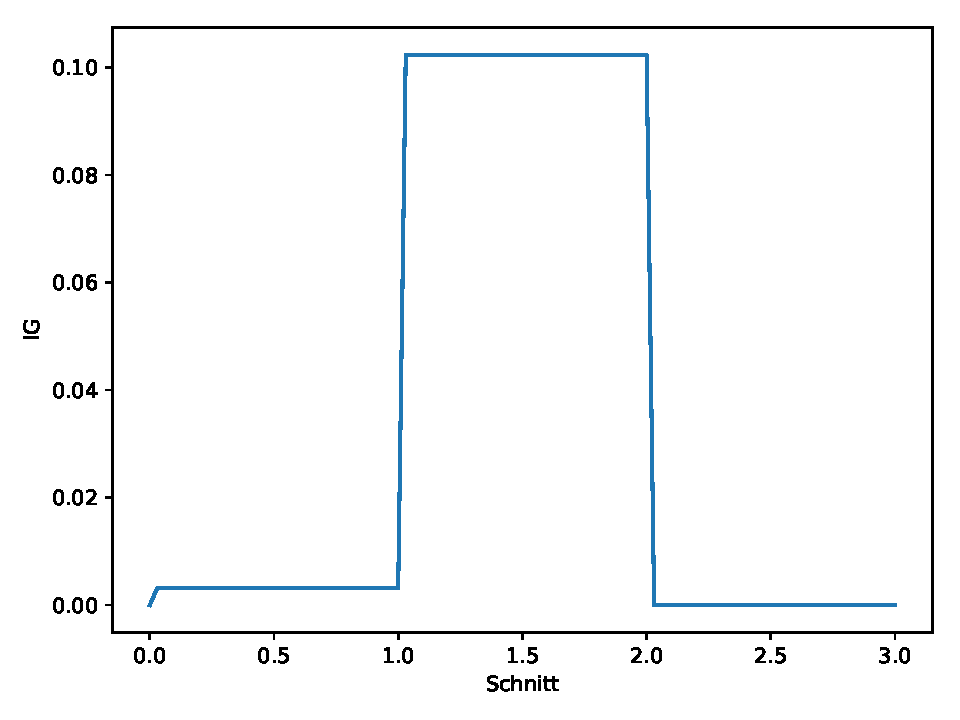
\includegraphics[scale=0.7]{IG_Wetter.pdf}
  \caption{Informationsgewinn aus dem Wetters in Abhängigkeit des Schnitts.}
  \label{abb:1}
\end{figure}
\begin{figure}
  \centering
  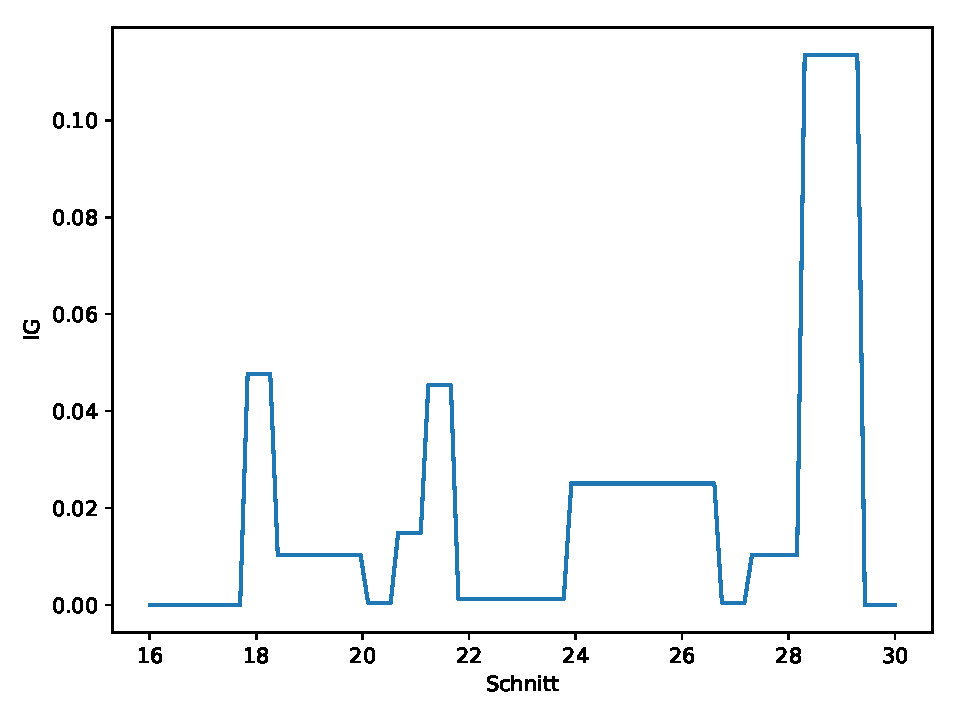
\includegraphics[scale=0.7]{IG_Temperatur.pdf}
  \caption{Informationsgewinn aus der Temperatur in Abhängigkeit des Schnitts.}
  \label{abb:2}
\end{figure}
\begin{figure}
  \centering
  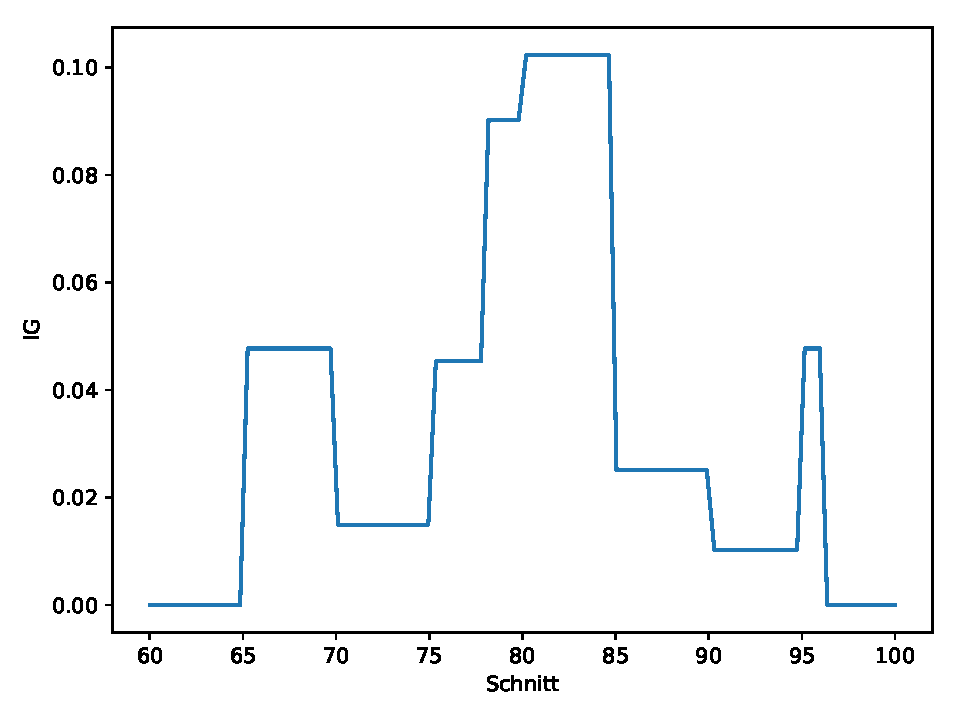
\includegraphics[scale=0.7]{IG_Luft.pdf}
  \caption{Informationsgewinn aus der Luftfeuchtigkeit in Abhängigkeit des Schnitts.}
  \label{abb:3}
\end{figure}

\subsection{d)}
Am besten eignet sich das Attribut "Temperatur" zur Trennung der Daten, da
hier bei einem Schnitt von etwa \SI{28,303}{\celsius} ein globaler, maximaler
Informationsgewinn von 0,1134 zu erkennen ist. Bei den anderen
Attributen ist des maximale Informationsgewinn geringer.


\begin{table}
  \centering
  \caption{Maximaler Informationsgewinn der Attribute}
  \label{tab:1}
  \begin{tabular}{c c c}
    \toprule
    Attribut & maximaler Informationsgewinn & Schnittstelle \\
    \midrule
    Wetter & 0,1022 & 1,03 \\
    Temperatur & 0,1134 & \SI{28,303}{\celsius} \\
    Luftfeuchtigkeit & 0,1022 & \SI{80,2020}{\percent} \\
    \bottomrule
  \end{tabular}
\end{table}

Zwar sind die Schnittstellen hier absolute Werte, aber man hat natürlich
einen bestimmten Bereich (zwischen zwei Werten), bei der die Schnittstelle
gesetzt werden kann, daher kommen auch die Plateaus in den Plots.
